\section{Statics and Mechanics of Materials}

\begin{center}
    Notes from \textbf{MECHENG 211: Introduction to Solid Mechanics}

    Taken at University of Michigan, Winter 2025
\end{center}

\subsection{Static Equilibrium} %% Chapter 1-5/6

A force $\vec{F}$ creates a \textbf{moment} about a point if it is located a distance $\vec{r}$ from the line of action of the $\vec{F}$. The moment $\vec{M}$ of a force is perpendicular to both $\vec{F}$ and $\vec{r}$, so in two dimensions, $\vec{M}$ necessarily points into or out of the page and is given by \[M = Fr\] In three dimensions, moments are computed by a cross product. For a moment about a point $A$ produced by a force acting at point $B$, the moment $\vec{M}_A$ is given by \[\vec{M}_A = \vec{r}_{AB}\times \vec{F} = (\vec{r}_B-\vec{r}_A)\times \vec{F}\]

A body is in \textbf{static equilibrium} if it does not translate or rotate. For this to be the case, the vector sum of the forces acting on the body must be zero, and the vector sum of the moments about any point on the body must also be zero. 

At each \textit{support} contacting a body, the body produces a \textit{reaction force}. For a body to be fully constrained, there must be as many reaction forces as \textit{degrees of freedom}. In two dimensions, there are \textit{three degrees of freedom} ($x$ and $y$ translation, and a moment). In three dimensions, there are \textit{six degrees of freedom} (translation in $x$ $y$, $z$, and moments in $x$, $y$, and $z$).

Most supports fall into one of the following categories:
\begin{enumerate}
    \item[] \textbf{Fixed support}. Sometimes called a built-in support. Constrains motion and rotation in all directions and therefore produces reaction forces and reaction moments in all directions.
    \item[] \textbf{Pin support}. Constrains translational motion while allowing free rotation, therefore producing reaction forces in the horizontal and vertical directions. Pin supports may often be used to approximate joints in structures like beams and trusses.
    \item[] \textbf{Simple support}. Prevents motion normal to the point of contact, producing a single reaction force. This joint is mathematically equivalent to a roller.
\end{enumerate}

When bodies come into contact through \textit{compressive forces}, a frictional force $F$ opposes motion. The magnitude of frictional force is generally given by the inequality $|F| < \mu N$. \textit{Incipient slip} refers to the force required to begin motion of a body, occurring when the frictional forces have just barely been overcome.

\subsection{Composite Structures}

It is possible to analyze a complicated, multi-element structure by breaking it into its components and supports. Such analysis involves drawing a free body diagram for each part, with external forces and reaction forces (and their 3rd Law reaction) listed at their appropriate positions and supports. Because the entire structure is in static equilibrium, each component must also be in static equilibrium and the forces on each component must thus satisfy the static equilibrium conditions.

A \textit{two-force member} is any component loaded at only two points, such as a support member in a truss. In this case, \[\vec{F}_A + \vec{F}_B = \vec{0},\hspace{0.5in} \vec{r}_{AB}\times \vec{F}_B = \vec{0}\] so $\vec{F}_A = -\vec{F}_B$ and thus forces act \textit{along a single line} through the component. If the forces point outwards, the member is in \textbf{tension}; if the forces point inwards, the member is in \textbf{compression}.
\newpage
There are two main ways to analyze the internal forces in a determinate structure, such as a truss:
\begin{enumerate}
    \item[] \textbf{Method of Pins}. Most useful for solving systems where many or all internal forces are to be calculated. Steps: \begin{enumerate}
        \item[1.] Separate structure into separate two-force members.
        \item[2.] Draw free-body diagrams for each two-force member, approximating joints as pins with reaction forces pointing away (in tension, which is positive by convention).
        \item[3.] Solve the force balance for the desired internal forces. This involves (at most) an $x$ and $y$ force balance for each member.
    \end{enumerate}
    \item[] \textbf{Method of Sections}. Most useful for solving systems where only some internal forces need to be known. Steps:
    \begin{enumerate}
        \item[1.] Cut a section through the body, cutting through at most three elements with unknown internal forces. The internal forces from cut members become external forces for the remaining section.
        \item[2.] Draw a free-body diagram for the section in question, with unknown forces pointing away from cut members (in tension, which is positive by convention).
        \item[3.] Solve the force and moment balance for the section. Since the entire body is in equilibrium, the section must also be in equilibrium. This involves setting net forces in $x$ and $y$ and net moment equal to zero.
    \end{enumerate}
\end{enumerate}

Each section of a loaded body must experience internal reactions which balance the external forces and moments. If one were to make a cut through any section of the body, these reactions would be exactly what is required to support either section of the cut.

By convention, the internal reactions include a normal force $N$ acting perpendicular to the cut, a shear force $V$ acting parallel to the cut, and a moment $M$. The internal reactions have opposite orientations on opposite sides of the cut.

In three dimensions, there is a single normal vector $\vec{N}$, two directional components to $\vec{V}$ (i.e. $x$ and $y$), and three rotational components (a bending moment $\vec{M}$ about the $x$ and $y$ axis, and a twisting torque $T$ about the $z$ axis).

\subsection{Stress and Strain}

In general, \textbf{stress} refers to the force acting over an area on a body (i.e. a "pressure" over a surface), and \textbf{strain} refers to the deformation of the body. Normal stress is denoted $\sigma$ and shear stress is denoted $\tau$.

Given a normal force $N$ acting uniformly on an area $A$, the normal stress at the section is given by \[\sigma = \frac{N}{A}\] Moments may also impart a normal stress. In particular, for a bar with cross-sectional area $A$ and area moment of inertia $I_x$, there is an additional component of stress given by \[\sigma_{zz} = \frac{M_xy}{I_x} - \frac{M_yx}{I_y}\] where $x$ and $y$ are taken from the centroid $c=(\overline{x},\overline{y})$. Similarly, given a uniform shear force $V$, the (average) shear stress is given by \[\tau = \frac{V}{A}\] and torque on a bar can also produce additional shear stress: \[\tau = \frac{Tr}{J}\]

\newpage

Stress acting on a body produces a \textbf{strain}, or change in the dimensions of an object. When a bar is loaded with a tensile force, it may experience some extension from its initial length $L_0$, given by $\delta = L-L_0$. \textit{Normal strain} $\varepsilon$, or \textit{extensional strain}, is defined as the ratio of extension and initial length, given by \[\varepsilon = \frac{\delta}{L_0}\]

\textit{Shear strain} acting on a body is simply computed as the total change of angle $\phi_1$ with respect to the horizontal and $\phi_2$ with respect to the vertical: \[\gamma = \phi_1 + \phi_2\]

\textbf{Hooke's Law} may be generalized to any material, and directly relates stress and strain. \begin{shaded}
    \textbf{Multiaxial Hooke's Law}. For a material which is elastically (linearly) deformed, the strains on a material relate directly to the stresses acting on the material by Hooke's Law:

    \[\epsilon_x = \frac{\sigma_x}{E} - \frac{\nu\sigma_y}{E} - \frac{\nu \sigma_z}{E} + \alpha\Delta T\]
    \[\epsilon_y = \frac{\sigma_y}{E} - \frac{\nu\sigma_x}{E} - \frac{\nu \sigma_z}{E} + \alpha\Delta T\]
    \[\epsilon_z = \frac{\sigma_z}{E} - \frac{\nu\sigma_x}{E} - \frac{\nu \sigma_y}{E} + \alpha\Delta T\]

    Here, $E$ is Young's Modulus, and $\alpha$ is the coefficient of thermal expansion. Both are specific to a material. $\nu$ is \textbf{Poisson's Ratio}, the ratio by which compression in one direction results in extension in another, and is related to $E$ and $G$ by the relationship \[\nu = -\frac{\epsilon_\text{lateral}}{\epsilon_\text{axial}} = \frac{E}{2G} - 1\] More concisely, \[E = 2G(1+\nu)\] 
\end{shaded}

If a problem is \textit{statically indeterminate} (more unknowns than equations), another equation may be found by considering the extension or torsion in the body. In particular, for a beam built in at both ends, extension of the beam must be zero (both ends are fixed), giving a relation between forces. The same applies for a bar in torsion, with a relation between torques.

Extension is associated with normal strain. For a bar with area $A$, Young's Modulus $E$, and initial length $L_0$, the extension is given by: \[\delta = \frac{FL_0}{AE}\] 

A bar loaded with a torque $T$ has an analogous relationship to the extension of a bar. The angle of torsion, $\phi$, is given by \[\phi = \frac{TL}{JG}\] where $G$ is the shear modulus for a material and $J$ is the \textit{second moment of inertia}. For a cylindrical bar in torsion, the relation between torque, shear, and angle of torsion is as follows: \[\frac{T}{J} = \frac{\tau_{z}}{r}=G\frac{\phi_B-\phi_A}{L_{AB}}\]

\newpage

Thin-walled pressure vessels have an internal pressure $P$ (i.e. due to an internal gas or fluid) and a wall of thickness $t$, where $t$ is negligible compared to radius $r$.

\begin{enumerate}
    \item[] \textbf{Cylindrical pressure vessels}. Internal pressure $P$ with a cap on either end. Stresses are given by \[\underbrace{\sigma_\theta = \frac{Pr}{t}}_\text{hoop stress, tangent to walls},\hspace{0.5in}\underbrace{\sigma_\text{axial} = \frac{Pr}{2t}}_\text{longitudinal stress, normal to cap}\]
    \item[] \textbf{Spherical pressure vessels}. Internal pressure $P$ with symmetric hemispheres. Stresses are given by \[\underbrace{\sigma_\theta = \sigma_\phi = \frac{Pr}{2t}}_\text{tangent to walls}\]
\end{enumerate}

Superposition allows the addition of normal and shear stresses. Stresses emerge from loads applied to a body. For a coordinate system oriented (facing the surface) with $z$ normal to the surface, $y$ up, and $x$ left:

\begin{enumerate}
    \item[] \textbf{Normal stress}. May be imparted due to a moment or normal force. \[\sigma_{zz} = \frac{N}{A} + \frac{M_xy}{I_x} - \frac{M_yx}{I_y}\]
    \item[] \textbf{Shear stress}. May be imparted due to a torque or a shear force. \[\tau_{zy} = \frac{V_y}{A},\ \tau_{zx} = \frac{V_x}{A},\ \underbrace{\tau_{z\theta} = \frac{Tr}{J}}_\text{may be in $x$ or $y$}\]
\end{enumerate}

Note that other forces may be present, i.e. hoop stress or longitudinal stress if a pressure vessel is contributing support. It is necessary in such cases to identify the coordinate directions of any such stresses.

\subsection{Transformation of Stress and Strain}

For any element experiencing stresses, there exists a coordinate transformation to a \textit{principal axis} where all stress is normal stress and another transformation where all stress is shear stress. These axes are normal to each other. Fracture is most likely to occur along one of these axes, depending on the nature of the material.

In general, if an element experiences coordinate stresses $\sigma_x$, $\sigma_y$, and $\tau_{xy}$, then the stress in a new axis an orientation $\theta$ away is given by \[\sigma_{x'} = \frac{\sigma_x + \sigma_y}{2}+ \frac{\sigma_x - \sigma_y}{2}\cos 2\theta + \tau_{xy}\sin2\theta\]
    \[\sigma_{y'} = \frac{\sigma_x + \sigma_y}{2} - \frac{\sigma_x - \sigma_y}{2}\cos 2\theta - \tau_{xy}\sin2\theta\]
    \[\tau_{x'y'} = -\frac{\sigma_x -\sigma_y}{2}\sin2\theta + \tau_{xy}\cos2\theta\]

The stresses along the \textit{principal axis} may be found from these equations: \[\sigma_{1,2}=\frac{\sigma_x+\sigma_y}{2}\pm \sqrt{\left(\frac{\sigma_x-\sigma_y}{2}\right)^2 + \tau_{xy}^2}\] where $\sigma_1>\sigma_2$. The maximum shear stress in the plane is given by \[\tau_\text{max} = \sqrt{\left(\frac{\sigma_x-\sigma_y}{2}\right)^2 + \tau_{xy}^2}\] 
\newpage
\textbf{Mohr's circle} is a visual representation which may be constructed to visualize planar stress. \begin{shaded}
    \textbf{Construction of Mohr's Circle}. Mohr's circle may be constructed by the following steps: 
    \vspace{-1em}
    \begin{enumerate}
        \item Create coordinate axes, by convention positive stress to the right and positive shear to the bottom.
        \item Plot the center of the circle at $\frac{\sigma_x+\sigma_y}{2}$.
        \item Draw the circle with radius $\sqrt{\left(\frac{\sigma_x-\sigma_y}{2}\right)^2+\tau_{xy}^2}$.
        \item Optionally, plot the reference stresses $(\sigma_{x},\tau_{xy})$ as a reference point $\theta=0$. The angle $\theta_p$ to the principal axes may be determined by trigonometry.
    \end{enumerate}
\end{shaded}


Mohr's circle is drawn graphically as so: \begin{center}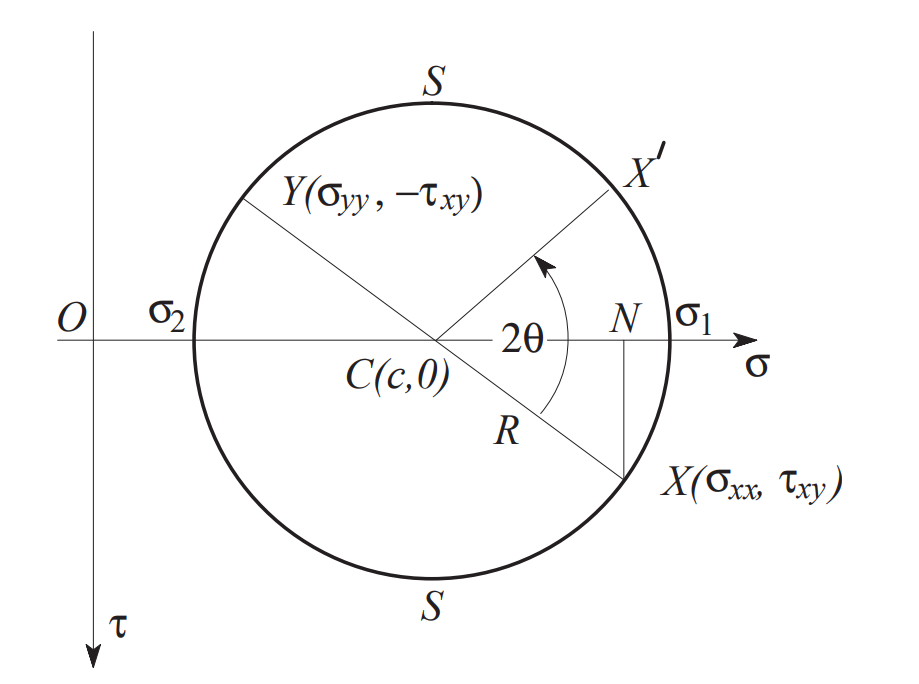
\includegraphics[scale=0.5]{Images/statics_mohrs.png}\end{center}

Since stress and strain are related by Hooke's Law, a Mohr's Circle may also be constructed for strain. The transformation equations are analogous to the stress transformations: \[\epsilon_{x'} = \frac{\epsilon_x + \epsilon_y}{2} + \frac{\epsilon_x-\epsilon_y}{2}\cos(2\theta) + \frac{\gamma_{xy}}{2}\sin(2\theta)\]
    \[\epsilon_{y'} = \frac{\epsilon_x + \epsilon_y}{2} - \frac{\epsilon_x-\epsilon_y}{2}\cos(2\theta) - \frac{\gamma_{xy}}{2}\sin(2\theta)\]
    \[\frac{\gamma_{x'y'}}{2} = - \frac{\epsilon_x-\epsilon_y}{2}\sin(2\theta) + \frac{\gamma_{xy}}{2}\cos(2\theta)\]

Principle strains also have an analogous transformations, and thus Mohr's circle is constructed in effectively the same manner for strains as with stresses:

\[\epsilon_{1,2} = \frac{\epsilon_x+\epsilon_y}{2}\pm \underbrace{\sqrt{\left(\frac{\epsilon_x-\epsilon_y}{2}\right)^2 + \left(\frac{\gamma_{xy}}{2}\right)^2}}_{\gamma_{\text{max}}/2}\]

It is important to note that, for planar stresses, $\sigma_3 = \sigma_z = 0$, but this is \textit{not the case} with planar strains, as a strain in one direction also causes strain in the others.

By using a \textit{strain gauge}, which measures electrical resistance (and thus strain, as electrical resistance increases with strain), the strain in a particular direction is related as follows:

\[\epsilon_a = \epsilon_x\cos^2\theta_a + \epsilon_y \sin^2\theta_a + \gamma_{xy}\sin\theta_a\cos\theta_a\]

Here, $\epsilon_a$ is read by the gauge and is thus known, and $\theta_a$ is known by the position of the strain gauge, so there are three unknowns. Thus, a strain gauge \textit{rosette}, with at least three strain gauges in unique directions, is required to find all the principal strains.

\subsection{Beam Deflection}

A loaded beam experiences some deflection, $u(z)$, as a function of the distance $z$ along the beam. For relatively small deflections, the following relationship holds: \[\frac{M(z)}{EI} = \frac{d\theta}{dz} = \frac{d^2u}{dz^2}\] $EI$ is the rigidity of the beam, and $M$ may vary as a function of position $z$. Integration gives $\theta(z)$ and $u(z)$ with constants of integration. These constants may be determined by evaluating $\theta$ or $u$ at supports and considering the boundary conditions of each support. Common boundary conditions, for support at arbitrary position $z=L_0$, are outlined:
\begin{enumerate}
    \item[] \textit{Built-in support}. \(u(L_0) = 0,\ \theta(L_0)=0\)
    \item[] \textit{Simple support}. \(u(L_0) = 0,\ M(L_0) = 0\)
    \item[] \textit{Free end}. \(V(L_0) = 0,\ M(L_0) = 0\)
\end{enumerate}